\begin{ReasoningBox}[title=Time Series Forecasting] % 可以通过 title 参数修改标题
    % --- 第一部分：问题描述与图片 ---
    % \begin{minipage}[t]{0.58\textwidth}
    \begin{wrapfigure}{r}{0.5\textwidth}
        \centering
        % wrapfigure 通常顶部会有多余空白，使用负 vspace 向上提，让图片和第一行文字对齐
        \vspace{-20pt} 
        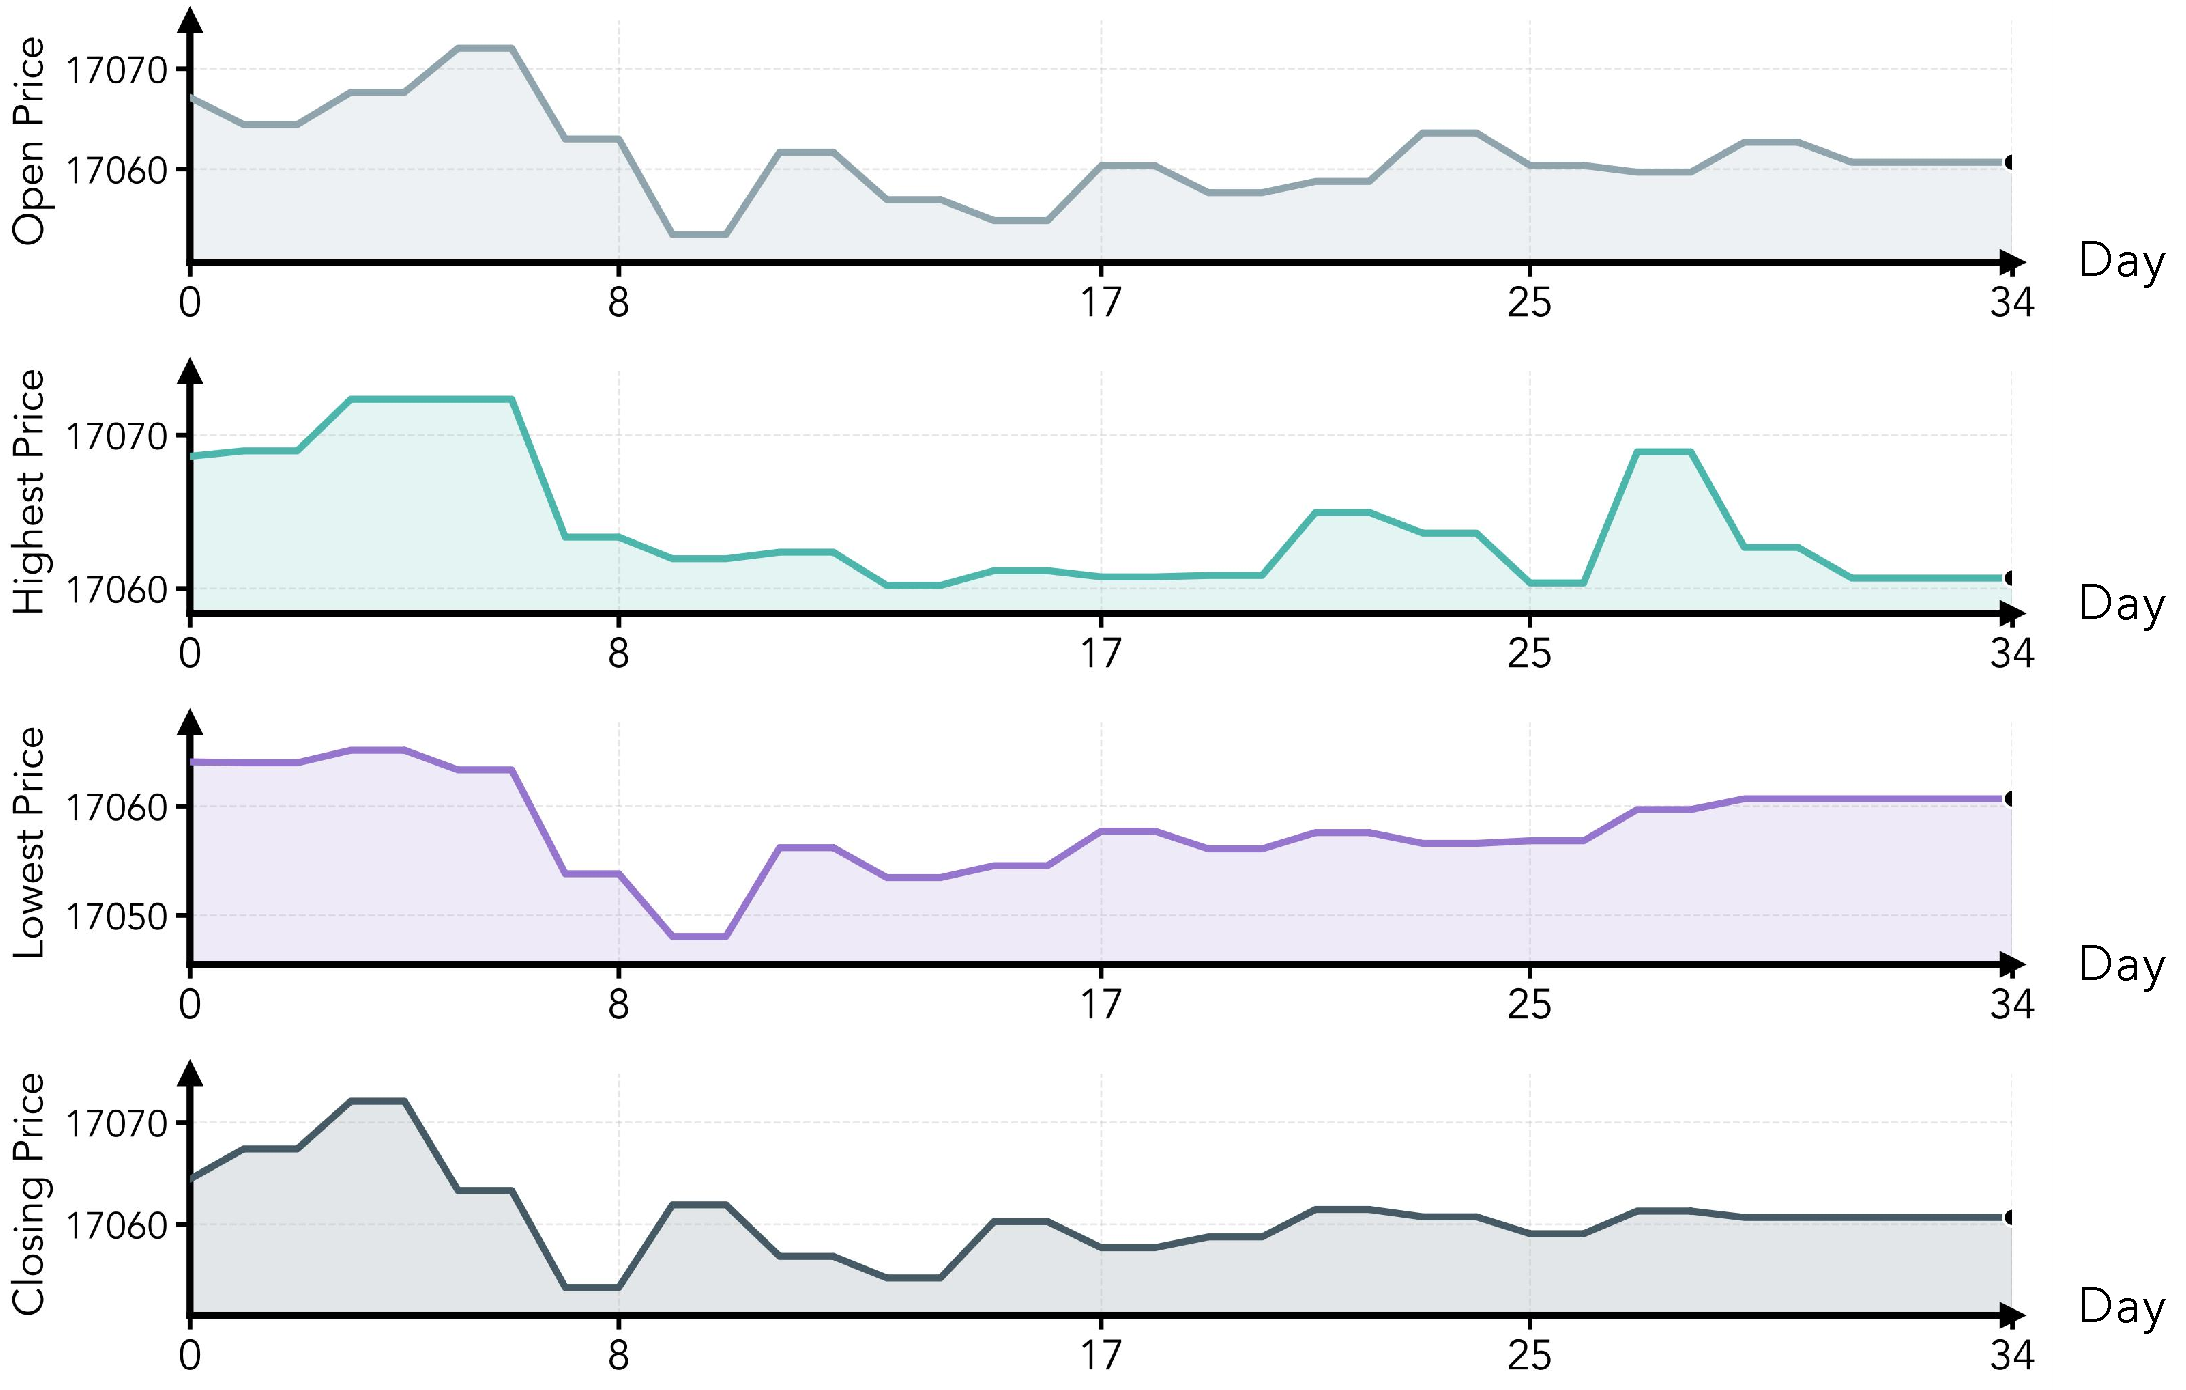
\includegraphics[width=\linewidth]{blocks/sample_cases_success/forecasting.pdf}
        % 调整底部的留白
        \vspace{-20pt}
    \end{wrapfigure}
\textbf{Question:} An event occurred affecting the Dow Jones Industrial Average (DJIA) stock index. The event summary is:

The overall PPI for final demand rose 0.4\% in June, following a 0.2\% decline in May. The index for final demand goods increased 0.5\%, while the index for final demand services rose 0.3\%. The stage 4 intermediate demand index rose 0.5\%, while the stage 3 intermediate demand index inched up 0.1\%. The stage 2 intermediate demand index moved up 0.4\%, and the stage 1 intermediate demand index increased 0.5\%.

The PPI for intermediate demand goods increased 0.4\% in June, driven by a 1.5\% increase in processed goods and a 0.9\% decrease in unprocessed goods. The PPI for services for intermediate demand climbed 0.6\%, driven by a 1.3\% increase in trade services and a 0.5\% rise in transportation and warehousing services.

The report also highlights the following key points:
\begin{itemize}
    \item The PPI for final demand goods increased 2.1\% over the past 12 months, while the index for final demand services rose 2.1\%.
    \item The PPI for energy goods increased 2.9\% over the past 12 months, while the PPI for food products increased 3.5\%.
    \item The PPI for industrial materials, excluding food and energy, increased 1.5\% over the past 12 months.
    \item The PPI for construction materials, such as lumber, plywood, and paper products, increased 1.4\% over the past 12 months.
    \item The PPI for machinery and equipment, such as motor vehicle parts, aircraft engines and parts, and medical devices, increased 1.3\% over the past 12 months.
\end{itemize}

The report also provides an overview of the prices of goods and services produced by domestic industries in the United States, covering sectors such as insurance, real estate, rental and leasing, professional services, employment, travel, security, cleaning, waste management, healthcare, education, accommodation, food, repair, entertainment, wholesale, retail, metal treatment, mining, and construction.

The report shows that the overall PPI increased by 1.4\% in June 2009 compared to the previous month, and by 4.3\% compared to the same period in the previous year. The index for insurance and annuities increased by 1.7\% in June 2009, while the index for real estate services increased by 4.0\%. The index for rental and leasing of goods decreased by 0.2\%, while the index for professional services increased by 2.1\%.

Overall, the PPI report suggests a moderate pace of inflation, with prices rising across various categories, including goods and services. The report provides valuable insights for businesses, policymakers, and investors to understand inflationary pressures and make informed decisions.

You are provided with the historical multivariate time series data for the 35 days leading up to and including the event day. Based on the historical data and the event context, which of the following options represents the most plausible trend for the \textit{Closing} price over the next 35 days? Please choose the list of values that best corresponds to the predicted future trajectory.

    \vspace{0.5em}

    % --- 第二部分：选项 ---
    \textbf{Answer Choices:} \\
    (A) 17092.76, 17093.24, 17093.24, 17090.95, 17090.95, 
17102.82, 17102.82, 17102.52, 17102.52, 17111.03, 17111.03, 17110.52, 17110.52, 17105.86, 17105.86, 17113.12, 17113.12, 17116.17, 17116.17, 17117.36, 17117.36, 17110.52, 17110.52, 17108.39, 17108.39, 17104.29, 17104.29, 17110.29, 17110.29, 17105.86, 17105.86, 17123.75, 17123.75, 17133.03, 17133.03 \\
    (B) 17084.81, 17084.81, 17094.09, 17094.09, 17111.98, 17111.98,
17107.55, 17107.55, 17113.55, 17113.55, 17109.45, 17109.45, 17107.32, 17107.32, 17100.48, 17100.48, 17101.67, 17101.67, 17104.72, 17104.72, 17111.98, 17111.98, 17107.32, 17107.32, 17106.81, 17106.81, 17115.32, 17115.32, 17115.02, 17115.02,
17126.89, 17126.89, 17124.60, 17124.60, 17125.08 \\
    (C) 17133.03, 17133.03, 17123.75, 17123.75, 17105.86, 17105.86,
17110.29, 17110.29, 17104.29, 17104.29, 17108.39, 17108.39, 
17110.52, 17110.52, 17117.36, 17117.36, 17116.17, 17116.17,
17113.12, 17113.12, 17105.86, 17105.86, 17110.52, 17110.52, 
17111.03, 17111.03, 17102.52, 17102.52, 17102.82, 17102.82,
17090.95, 17090.95, 17093.24, 17093.24, 17092.76 \\
    (D) 17133.03, 17133.03, 17142.31, 17142.31, 17160.20, 17160.20,
17155.77, 17155.77, 17161.77, 17161.77, 17157.67, 17157.67, 
17155.54, 17155.54, 17148.70, 17148.70, 17149.89, 17149.89,
17152.94, 17152.94, 17160.20, 17160.20, 17155.54, 17155.54, 
17155.03, 17155.03, 17163.54, 17163.54, 17163.24, 17163.24,
17175.11, 17175.11, 17172.82, 17172.82, 17173.30 \\
    \textbf{Correct Answer:} \textcolor{correctgreen}{(C)} \\
\end{ReasoningBox}